\begin{figure}[htbp]
\centering
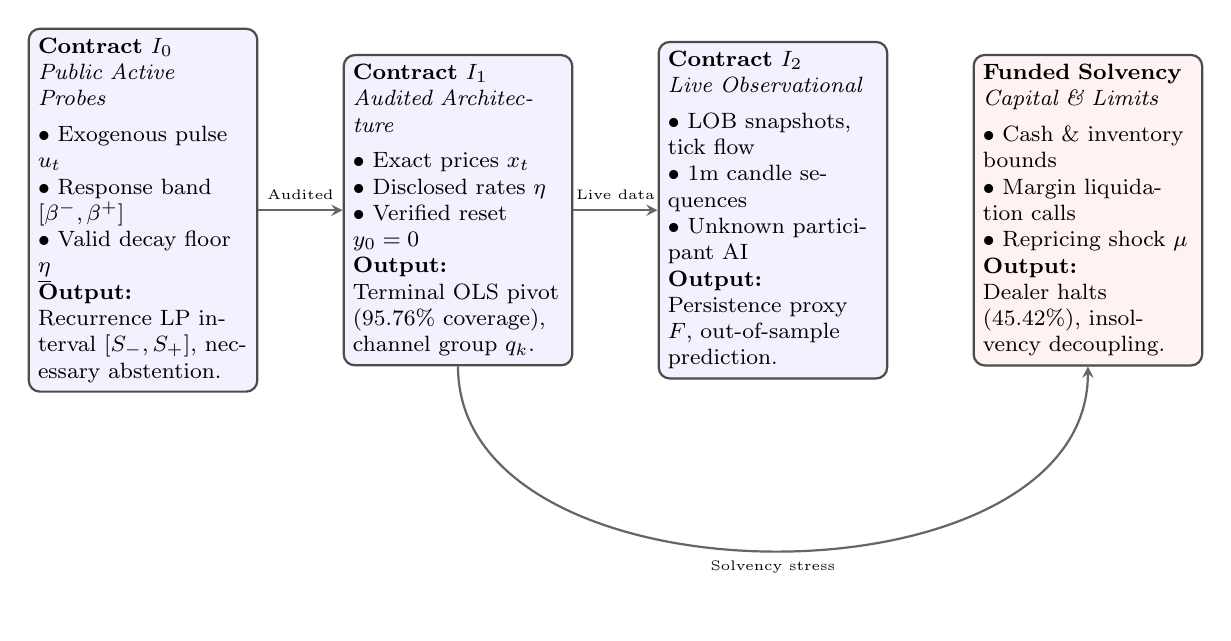
\begin{tikzpicture}[
  box/.style={rectangle, draw=black!70, thick, rounded corners, fill=blue!5, text width=0.22\textwidth, minimum height=3.5cm, align=left, font=\footnotesize},
  arrow/.style={->, >=stealth, thick, draw=black!60},
  header/.style={font=\bfseries\footnotesize, text=blue!80!black}
]
\node[box] (I0) at (0, 0) {
  \textbf{Contract $I_0$}\\
  \textit{Public Active Probes}\\[0.4em]
  $\bullet$ Exogenous pulse $u_t$\\
  $\bullet$ Response band $[\beta^-, \beta^+]$\\
  $\bullet$ Valid decay floor $\underline\eta$\\
  \textbf{Output:}\\
  Recurrence LP interval $[S_-, S_+]$, necessary abstention.
};

\node[box] (I1) at (4.0, 0) {
  \textbf{Contract $I_1$}\\
  \textit{Audited Architecture}\\[0.4em]
  $\bullet$ Exact prices $x_t$\\
  $\bullet$ Disclosed rates $\boldsymbol\eta$\\
  $\bullet$ Verified reset $y_0 = 0$\\
  \textbf{Output:}\\
  Terminal OLS pivot (95.76\% coverage), channel group $q_k$.
};

\node[box] (I2) at (8.0, 0) {
  \textbf{Contract $I_2$}\\
  \textit{Live Observational}\\[0.4em]
  $\bullet$ LOB snapshots, tick flow\\
  $\bullet$ 1m candle sequences\\
  $\bullet$ Unknown participant AI\\
  \textbf{Output:}\\
  Persistence proxy $F$, out-of-sample prediction.
};

\node[box, fill=red!5] (Funded) at (12.0, 0) {
  \textbf{Funded Solvency}\\
  \textit{Capital \& Limits}\\[0.4em]
  $\bullet$ Cash \& inventory bounds\\
  $\bullet$ Margin liquidation calls\\
  $\bullet$ Repricing shock $\mu$\\
  \textbf{Output:}\\
  Dealer halts (45.42\%), insolvency decoupling.
};

\draw[arrow] (I0.east) -- node[above, font=\tiny]{Audited} (I1.west);
\draw[arrow] (I1.east) -- node[above, font=\tiny]{Live data} (I2.west);
\draw[arrow] (I1.south) to[out=-90, in=-90] node[below, font=\tiny]{Solvency stress} (Funded.south);
\end{tikzpicture}
\caption{Information map: observational regimes, measurement contracts, and operational boundary limits.}
\label{fig:F1_information_map}
\end{figure}
